\chapter{Background}\label{chap:background}

This chapter presents all the background information needed to work on this thesis. It also describes all the modules needed for implementing this project. The following figure 
display the three main modules that describe the architecture of the project.

\begin{figure}[h!]
\centering
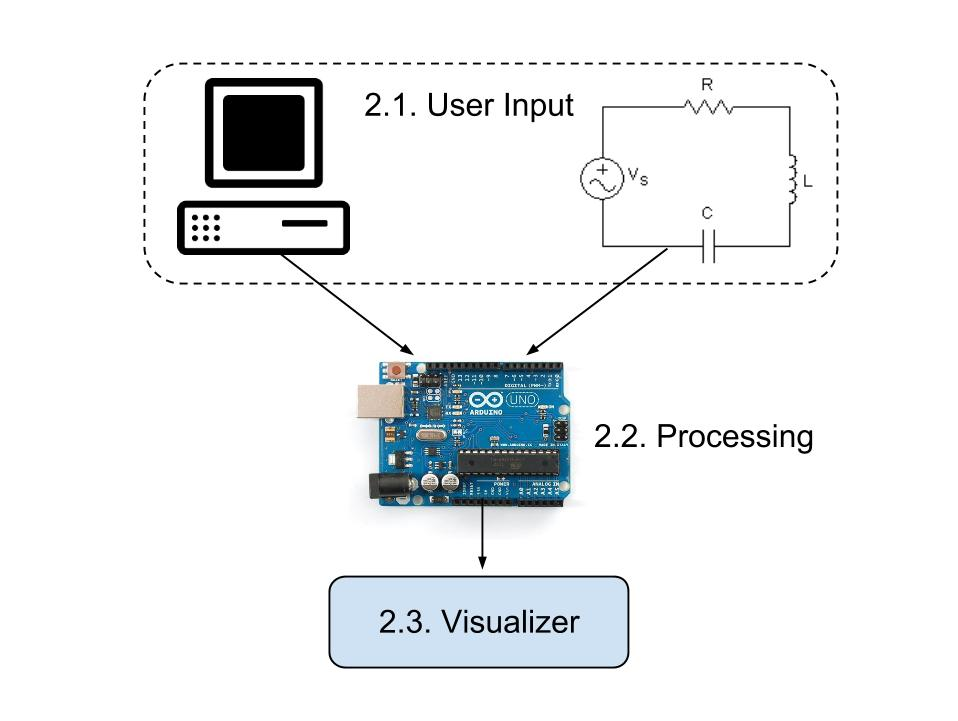
\includegraphics[height=9cm, width=12cm]{Architecture.jpg}
\caption{Virtual Arduino Architecture}
\label{Architecture}
\end{figure}

\section{User Input Modules}
This is the first level of the program’s architecture. It represents all forms of input the user can give. This input can be in the form of Arduino code or circuitry.

\subsection{Computer Module}
In this module the user writes arduino code and compile it through the Arduino IDE. Instead of uploading the code to the actual arduino, the user redirects the output to a virtual serial port from which the simulator reads. The code is sent in the form of a stream of bytes that is sent to the processing module. Our application simulate the two directional byte transfer process. It also simulates the \href{http://www.atmel.com/tools/STK500.aspx?tab=overview}{STK500} starter kit that communicates with the IDE in this process(Boatloader).

\subsection{Circuitry Module}
The hardware part of working with Arduino is described in this module. The user can build circuits and add hardware components to it. He can also connect these circuits to the Arduino through the Arduino ports.

\section{Processing Module}
This is the second level of the architecture which processes the inputs it receives from the first module. It sends these states to the visualizer module. This module is discussed later with more details in Chapter \ref{chap:implementation}.

\section{Output Visualizer}
In this module the user will be able to visualize the output of the code on the hardware components. This module uses the results from the previous module and make the behaviour changes visible on the Arduino board, circuitry and hardware components.

\subsection{Success Scenario Visualizer}
This part simulates the scenario when the code is compiled and uploaded and there are no hardware failures. Each component’s output is visualized. The user can modify the sensors input and accordingly the output changes.

\subsection{Hardware Failure Visualizer}
This is the case where failures are caused by hardware not the user. The user will be able to debug the circuits using a virtual avo-meter that is be implemented.


